% !TEX root = Master.tex

Unlike implicit copulas, \textit{explicit copulas} can be specified directly by taking into account certain constructional principles. The most important aspects of a such explicit copulas, in particular \textit{archimedean copulas}, are showcased in this subsection. Archimedian copulas are of the general form
\begin{equation}C(\boldsymbol{u})=\phi^{-1}\left(\phi\left(u_{1}\right)+\cdots+\phi\left(u_{d}\right)\right),
\label{eq:archimedean_copula_1}
\end{equation}
where the function $\phi:[0,1] \rightarrow [0, \infty)$ is the \textit{(archimedean) generator} and satisfies the following properties:
\begin{itemize}
\item $\phi$ is strictly decreasing in the entire domain $[0, 1]$
\item We set $\phi (1) = 0$
\item If  $\phi(0)=\lim \limits _{u \rightarrow 0^{-}} \phi(u)= \infty$, then $\phi$ is called \textit{strict}.
\end{itemize}




Based on \autoref{eq:archimedean_copula_1} and according to the form of the generator, we can construct several copula families. Three of the most popular ones are the \textit{Gumbel}, the \textit{Clayton} and the \textit{Frank} \textit{copula}, which are discussed for the bivariate case. The advantage of such copulas lies in the fact that they interpolate between certain fundamental dependence structures.\\

\begin{figure}[H]
\centering
  \includegraphics[width=.5\linewidth]{figures/archimedean_generator.eps}
  \caption{Shape of a generator function}
  \label{fig:archimedean_generator}
\end{figure}

\textbf{Clayton Copula}\\
If the generator takes on the form
\begin{equation}
\phi_{C l}(u)=\frac{1}{\theta}\left(u^{-\theta}-1\right)
\end{equation}
then we obtain the \textit{Clayton copula} given by
\begin{equation}
C_{\theta}^{C l}\left(u_{1}, u_{2}\right)=\left(\max \left\{u_{1}^{-\theta}+u_{2}^{-\theta}-1,0\right\}\right)^{-\frac{1}{\theta}},
\end{equation}
where $\theta \in[-1, \infty) \backslash\{0\}$.\\
For $\theta > 0$ the generator of the Clayton copula is strict and we arrive at 
\begin{equation}
C_{\theta}^{C l}\left(u_{1}, u_{2}\right)= (u_{1}^{-\theta}+u_{2}^{-\theta}-1)^{-\frac{1}{\theta}}.
\end{equation}

Note that for $\theta \rightarrow 0$ we obtain the independence copula.
\\
%Note that for $\theta=-1$, we obtain the lower Fr\'echet-Hoeffding bound $W$, whereas for the limits $\theta \rightarrow 0$ and $\theta \rightarrow \infty$ we arrive at the independence copula $\Pi$ and the comonotonicity copula $M$ respectively.


 \begin{figure}[H]
\centering
\begin{subfigure}{.45\textwidth}
  \centering
  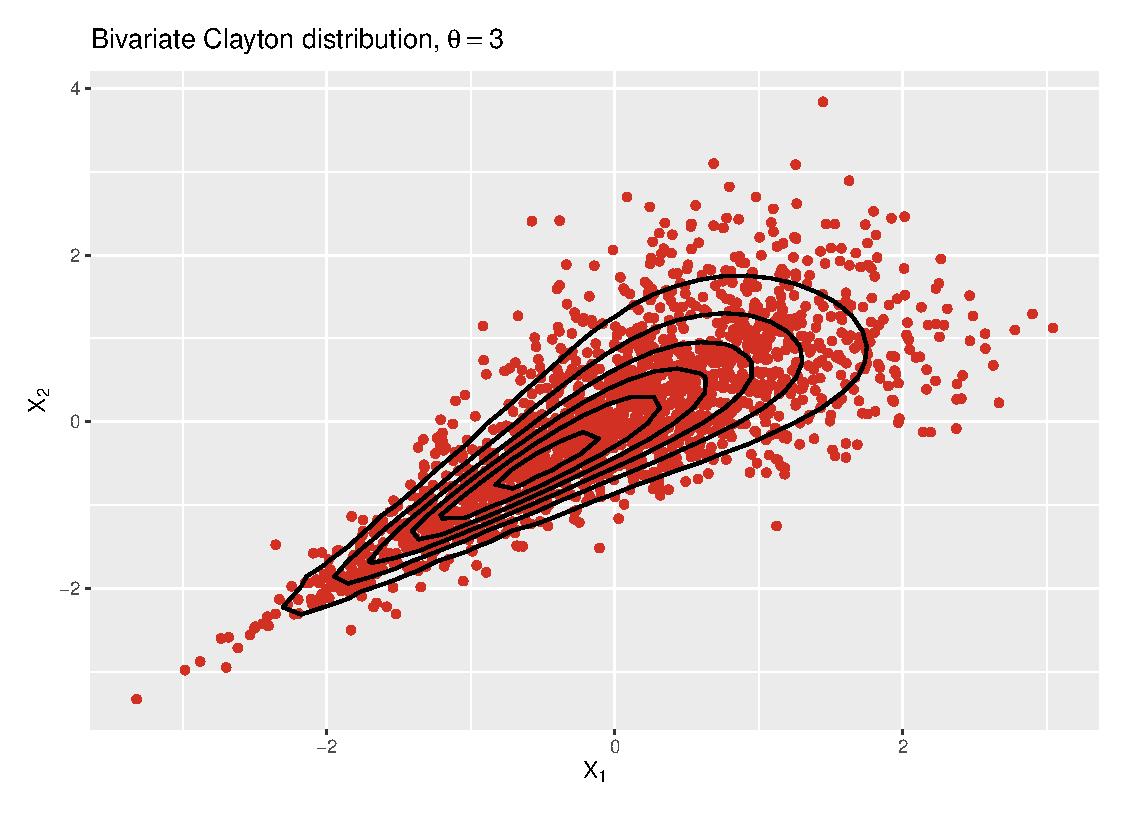
\includegraphics[width=\linewidth]{figures/bivariate_clayton.eps}
  \caption{Clayton distribution with contour lines}
  \label{fig:bivariate_clayton}
\end{subfigure}
\begin{subfigure}{.45\textwidth}
  \centering
  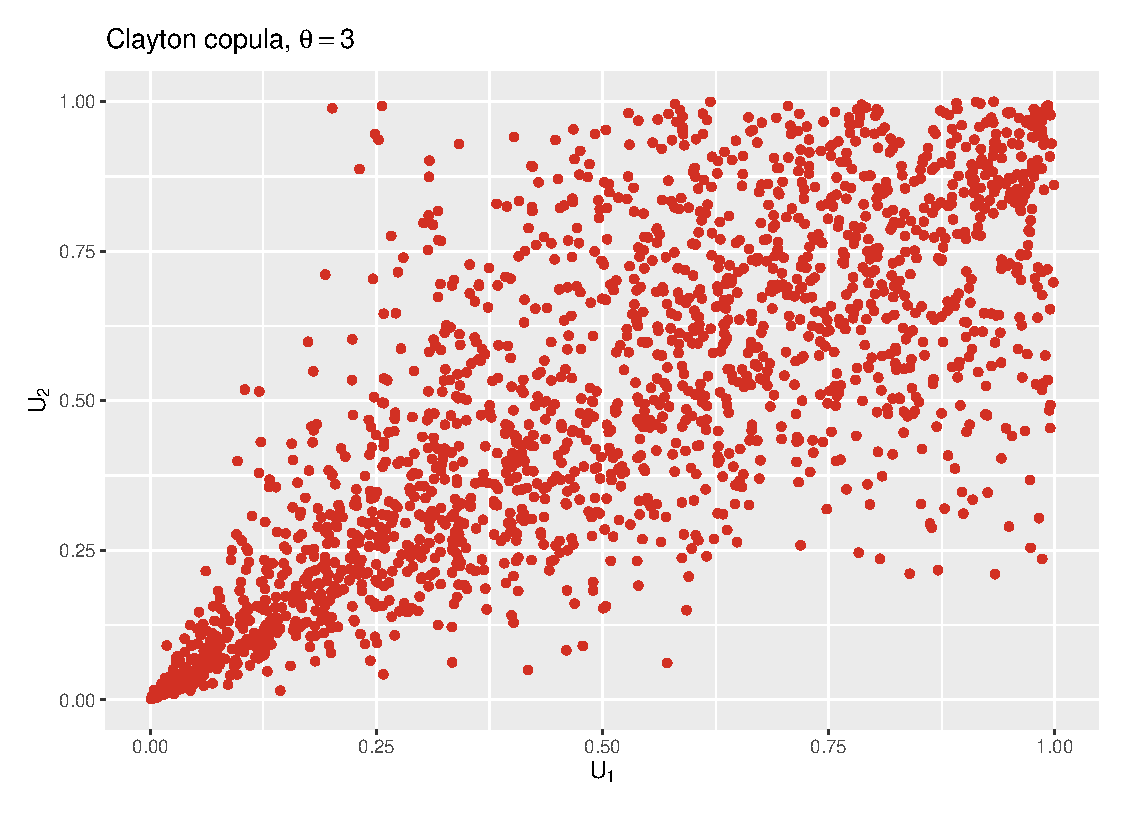
\includegraphics[width=\linewidth]{figures/clayton_copula.eps}
  \caption{Clayton copula}
  \label{fig:clayton_copula}
\end{subfigure}
\caption{Bivariate Clayton distribution and Clayton copula for Kendall's $\tau = 0.6$ and simulated sample of size $n = 1800$, both with standard normal margins}
\label{fig:clayton_plots}
\end{figure}




\textbf{Gumbel Copula}\\
If the generator takes on the form
\begin{equation}
\phi_{G u}(u)=(-\ln u)^{\theta}, \quad \theta \in [1, \infty),
\end{equation}
then we arrive at the \textit{Gumbel copula} given by
\begin{equation}
C_{\theta}^{G u}\left(u_{1}, u_{2}\right)=\exp \left[-\left(\left(-\ln u_{1}\right)^{\theta}+\left(-\ln u_{2}\right)^{\theta}\right)^{\frac{1}{\theta}}\right].
\end{equation}
Note that for $\theta= 1$, we obtain the independence copula $\Pi$.
% while for $\theta \rightarrow \infty$ the Gumbel copula converges to the comonotonicity copula $M$. 
Strictness holds for the entire parameter range of $\theta$.
\\

 \begin{figure}[H]
\centering
\begin{subfigure}{.45\textwidth}
  \centering
  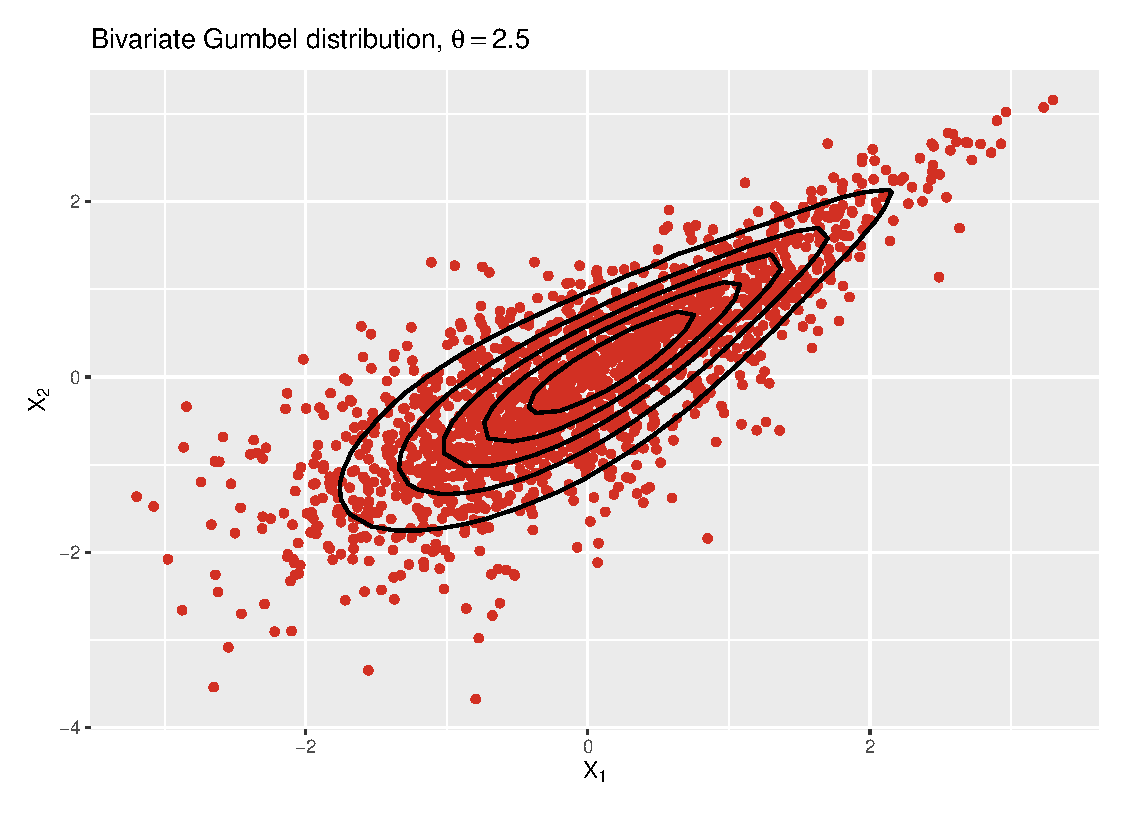
\includegraphics[width=\linewidth]{figures/bivariate_gumbel.eps}
  \caption{Gumbel distribution with contour lines}
  \label{fig:bivariate_gumbel}
\end{subfigure}
\begin{subfigure}{.45\textwidth}
  \centering
  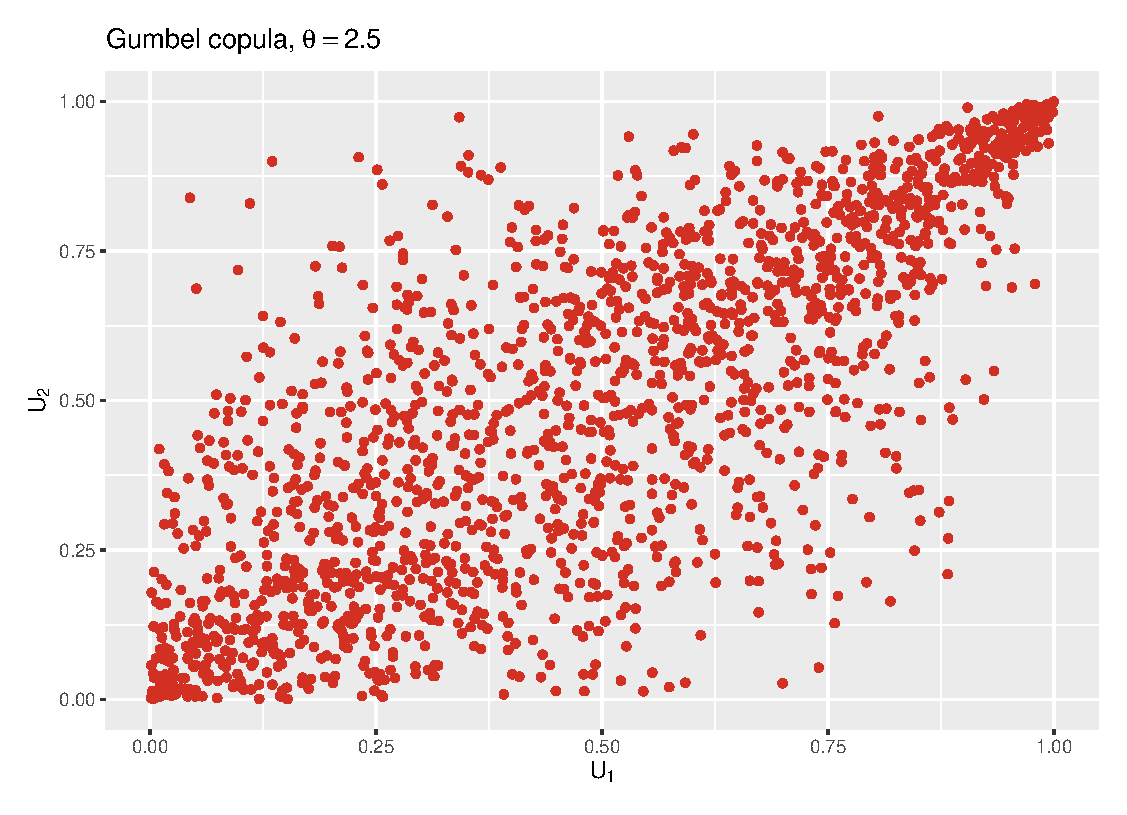
\includegraphics[width=\linewidth]{figures/gumbel_copula.eps}
  \caption{Gumbel copula}
  \label{fig:gumbel_copula}
\end{subfigure}
\caption{Bivariate Gumbel distribution and Gumbel copula for Kendall's $\tau = 0.6$ and simulated sample of size $n = 1800$, both with standard normal margins}
\label{fig:gumbel_plots}
\end{figure}



\textbf{Frank Copula}\\
If the generator takes on the form
\begin{equation}
-\ln \left(\frac{\mathrm{e}^{-\theta u}-1}{\mathrm{e}^{-\theta}-1}\right), \quad \theta \in \mathbb{R} \backslash\{0\},
\end{equation}
we obtain the \textit{Frank copula} given by
\begin{equation}
C_{\theta}^{F r}\left(u_{1}, u_{2}\right)=-\frac{1}{\theta} \ln \left(1+\frac{\left(e^{-\theta u_{1}}-1\right) \cdot\left(e^{-\theta u_{2}}-1\right)}{e^{-\theta}-1}\right).
\end{equation}

The Frank copula is strict in the parameter range of $\theta$ and it converges to the independence copula $\Pi$ if $\theta \rightarrow 0$.
\\

%The Frank copula is strict in the parameter range of $\theta$ and interpolates between $W$ ($\theta \rightarrow -\infty$), $\Pi$ ($\theta \rightarrow 0$) and $M$ ($\theta \rightarrow \infty$).

 \begin{figure}[H]
\centering
\begin{subfigure}{.45\textwidth}
  \centering
  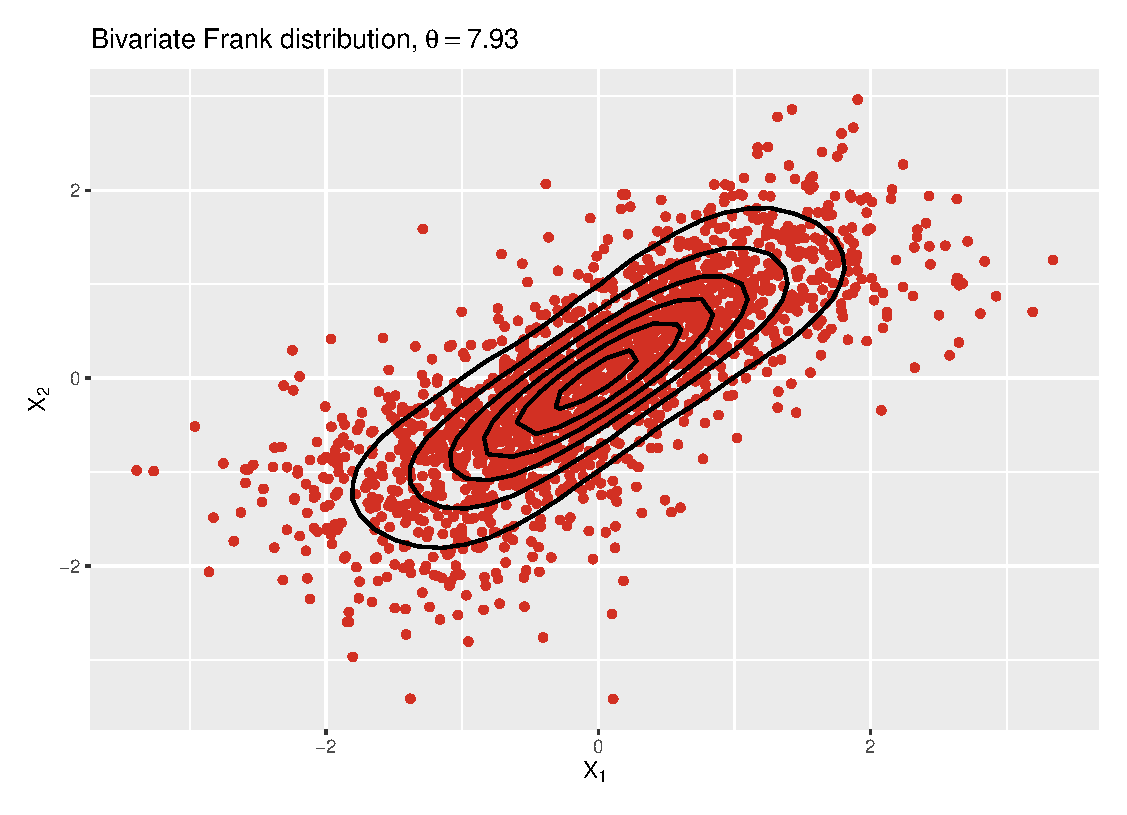
\includegraphics[width=\linewidth]{figures/bivariate_frank.eps}
  \caption{Frank distribution with contour lines}
  \label{fig:bivariate_frank}
\end{subfigure}
\begin{subfigure}{.45\textwidth}
  \centering
  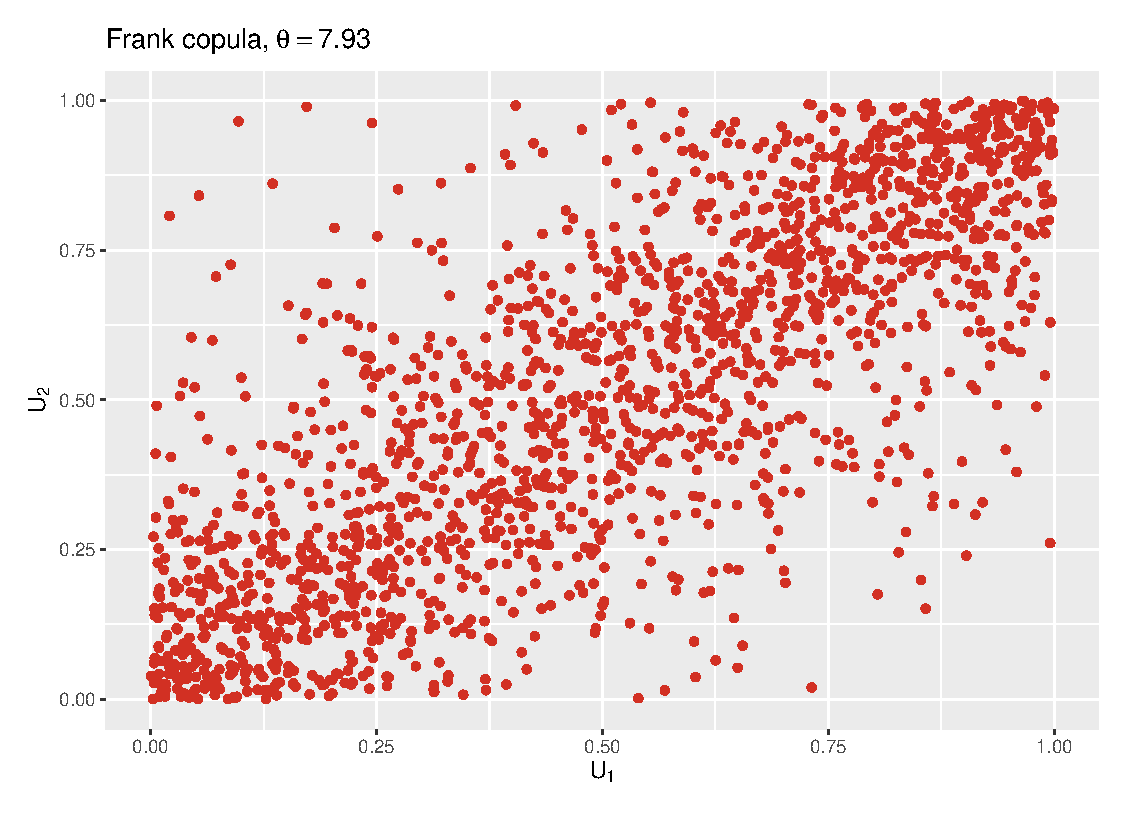
\includegraphics[width=\linewidth]{figures/frank_copula.eps}
  \caption{Frank copula}
  \label{fig:frank_copula}
\end{subfigure}
\caption{Bivariate Frank distribution and Frank copula for Kendall's $\tau = 0.6$ and simulated sample of size $n = 1800$, both with standard normal margins}
\label{fig:frank_plots}
\end{figure}





